\documentclass{article}
\usepackage{amsmath}
\usepackage{tikz}
\usepackage{pgfplots}
\pgfplotsset{width=3in,compat=1.9}
\usepackage[inline]{enumitem}  
\usepackage[letterpaper, total={7.5in, 10in}]{geometry}
\title{JPS Science League: AP Physics II}
\author{Kevin Yang and Elisha Zhao}
\date{Entrance Exam}
\makeatletter
% This command ignores the optional argument for itemize and enumerate lists
\newcommand{\inlineitem}[1][]{%
\ifnum\enit@type=\tw@
    {\descriptionlabel{#1}}
  \hspace{\labelsep}%
\else
  \ifnum\enit@type=\z@
       \refstepcounter{\@listctr}\fi
    \quad\@itemlabel\hspace{\labelsep}%
\fi}
\makeatother
\parindent=0pt
\begin{document}
	\maketitle
	\renewcommand{\labelenumii}{\alph{enumii})}
	\textbf{Instructions: }There are $25$ test questions that will determine your placement. You will be given $50$ minutes for this exam. Points will not be taken off for wrong answers so you are encouraged to answer every question. Suppose that $g=10\;\frac{m}{s^2}$. Good luck and have fun!
	\begin{enumerate}
		%Question 1: Understanding the meaning of PV diagram // Change?
		\item[1)]
		Kevin loves PV diagrams. Almost as much as he loves the Carnot cycle. Given the following PV diagram:
		%Add diagram
		\begin{center}
			\begin{tikzpicture}
				\begin{axis}[
	           		axis lines = left,
					title={Sample PV Diagram},
	    			xlabel= {$V(L)$},
	    			ylabel= {$P(atm)$},
                    xmin = 0,
	                xmax = 10,
                    ymin = 0,
                    ymax = 10,
                    samples = 100,
	    			]
					\addplot[
						domain = 1:3,
						color = blue,
					]
					{10/(x)};  
					\addplot[
						domain = 5:9,
						color = red,
					]
					{32/x};
				\end{axis}
			\end{tikzpicture}
		\end{center}
		Which of the following transition type is the blue curve:
		\begin{enumerate}
			\item
			\inlineitem 
			\inlineitem 
			\inlineitem
		\end{enumerate}
		%Question 2: PV Diagram - Carnot Cycle
		\item[2)]
		Kevin really loves Carnot cycles. In order to share his love of Carnot cycles with you, he decided to give you a Carnot cycle question. However, a Carnot cycle would be too simple so he decided to spice things up by changing a transition of the Carnot cycle. According to the diagram below:
		%Add diagram
		\begin{center}
			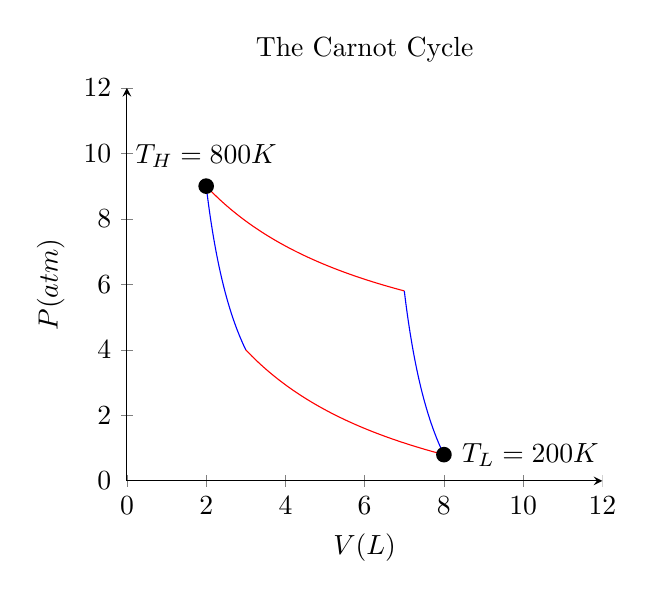
\begin{tikzpicture}
				\begin{axis}[
	           		axis lines = left,
					title={The Carnot Cycle},
	    			xlabel= {$V(L)$},
	    			ylabel= {$P(atm)$},
                    xmin = 0,
	                xmax = 12,
                    ymin = 0,
                    ymax = 12,
                    samples = 100,
	    			]
					\addplot[
						domain = 2:3,
						color = blue,
					]
					{10/(x-1)-1};  
					\addplot[
						domain = 2:7,
						color = red,
					]
					{32/(x+3)+2.6};
                    \addplot[
						domain = 7:8,
						color = blue,
					]
					{10/(x-6)-4.2};
                    \addplot[
						domain = 3:8,
						color = red,
					]
					{32/(x+2)-2.4};
                    \node[label = {90:{$T_H = 800K$}}, circle, fill, inner sep = 2pt] at (axis cs:2,9){};
                    \node[label = {0:{$T_L = 200K$}}, circle, fill, inner sep = 2pt] at (axis cs:8,0.8){};
				\end{axis}
			\end{tikzpicture}
		\end{center}
		What is the maximum amount of work that an engine running the proposed cycle can provide?
		\begin{enumerate}
			\item
			\inlineitem 
			\inlineitem 
			\inlineitem
		\end{enumerate}
	\end{enumerate}
	\textbf{Use the following information for Questions \#3 and \#4: }When Kevin was first learning thermodynamics, he was forced to memorize the following chart:
	%Chart of heat
	To share his pain, Kevin is making you fill out some missing parts of the chart. Nevertheless, it is a very important chart and Kevin suggests that you memorize it. Its not that bad.
	\begin{enumerate}
		%Question 3: Completing the heat chart
		\item[3)]
		On the chart, there is a missing square labeled $(A)$. Please use the already filling in information of the chart and prior knowledge to deduce what belongs in $(A)$.
		\begin{enumerate}
			\item
			\inlineitem 
			\inlineitem 
			\inlineitem
		\end{enumerate}
		%Question 4: Completing the heat chart
		\item[4)]
		Now that you have completed $(A)$, naturally $(B)$ comes next. Kevin promises that you don't need the answer of $(A)$ to find out what $(B)$ is. Anyways, what belongs in $(B)$.
		\begin{enumerate}
			\item
			\inlineitem 
			\inlineitem 
			\inlineitem
		\end{enumerate}
		%Question 5: Third Law of Thermodynamics
		\item[5)]
		 Kevin loves building stuff. One day after school he was hanging out with his friends(which he has a lot of btw) and accidentally built a way. This wall was extremely long, thick and magnificent. It was the best wall that he had ever laid eyes on.  Normally, temperatures in NJ go up to as much as $110^o$F. The proposed wall has entropy, in fact, a lot of entropy. Which of the following objects would have the least entropy?
		\begin{enumerate}
			\item An sphere at $0\;K$
			\inlineitem  A crystal at $0\;K$
			\inlineitem  A sphere at infinite $K$
			\inlineitem	 A box at room temperature
		\end{enumerate}
		%Question 6: Ideal gas law
		\item[6)]
		Elisha was working with ideal gases for a science experiment that she was designing. More specifically, she used a monoatomic ideal gas-meaning that there is only one atom per molecule. The gas was initially at a temperature of $23^o$C, pressure of $2.3\;atm$, and a volume of $2.2\;L$. Elisha raises the temperature to $45^o$C and allows the pressure to decrease to $0.9\;atm$. What is the new volume of the gas?
		\begin{enumerate}
			\item
			\inlineitem 
			\inlineitem 
			\inlineitem
		\end{enumerate}
		%Question 7: Kinetic Theory
		\item[7)]
		What even is kinetic theory
		\begin{enumerate}
			\item
			\inlineitem 
			\inlineitem 
			\inlineitem
		\end{enumerate}
	\end{enumerate}
	\textbf{Use the following information for Questions \#8 and \#9: }After reading the problems that he wrote, Kevin realized that he is quite narcissistic for using his himself has the main character in all but one question so far. Thus, Kevin wishes to wash these sins off using water. To do so, Kevin designs a shower system. All of the water comes from a water tank placed $20\;m$ into the air. A pipe, placed perpendicular to the ground, with a diameter of $20\;cm$ brings the water down to Kevin's head level of $2\;m$. Before water arrives at the shower head, the $20\;cm$ pipe smoothly becomes a pipe with a diameter of $10\;cm$. Suppose that every component is frictionless, all curves are completely smooth and curved so no energy will be lost and the viscosity of water is negligible.
	\begin{enumerate}
		%Question 8: Fluid Dynamics
		\item[8)]
		Can you help find out how fast the water will be washing Kevin's sin off at?
		\begin{enumerate}
			\item
			\inlineitem 
			\inlineitem 
			\inlineitem
		\end{enumerate}
		%Question 9: Fluid Statics
		\item[9)]
		As Kevin was washing off his body, he soon got bored and decided to bring out his rubber ducky. His rubber ducky was not really rubber at all. It was made of a quiet heavy material with a relative density of $0.25$. It was shaped like a ducky either. It was more like a rectangular prism with dimensions with a base of $20\;m x 43\;m$ and a height of $25\;m$.(Yeah, its a huge duck. Get over it). Kevin places the rubber ducky base first into his bath tub, which happens to be quite large too and wants to know how much of the rubber ducky is above water. Can you help him figure out in meters, how much of the rubber ducky is above water?
		\begin{enumerate}
			\item
			\inlineitem 
			\inlineitem 
			\inlineitem
		\end{enumerate}
		%Question 10: Fluid Statics
		\item[10)]
		Both Elisha and Kevin has Mr. Mac as a teacher for physics. There was an interesting concept that they learned in class about liquids that Elisha wanted to try out for herself. More commonly known as the hydrolic press/lifter, this device utilizes Pascal's Law to lift different items. She has set up different kinds of hydrolic presses in order to lift different items. Check diagram below. The first press, $A$, has an input surface with a radius of $23\;cm$ and a output surface of $78\;cm$; it is lifting a mass of $30\;kg$. The second press, $B$, has an input surface with a radius of $47\;cm$ and a output surface of $83\;cm$; it is lifting a mass of $54\;kg$. The third press, $C$, has an output surface with a radius of $34\;cm$ and an output surface of $11\;cm$; it is lifting a weight of $7\;kg$. Can you help Elisha rank the forces that she needs to exert on the presses from greatest to least?
		\begin{enumerate}
			\item
			\inlineitem 
			\inlineitem 
			\inlineitem
		\end{enumerate}
		%Ideal Gases
		\item[11)]
		H3h3's Ethan is often sporting a sign of VN in his pictures. This alludes to a very interesting activity that became popularized after the negative effects of tar in lungs became apparent. In the scientific community, this behavior is referred to the inhalation of water vapor. For the purpose the problem, let us assume that water molecules are diatomic(just ignore one of those teeny weeny little Hydrogens). Kevin was able to gather$1000\; Pa$ in a container with dimensions of $15\;m$ x $20\;m$ x $10\;m $ with a piston attached at $STP$. The walls of the container is perfected insulative so there is no heat transfer between the outside environment and the gas inside the container. While moving the container around, Kevin accidentally bumped the piston to make the dimensions of the container $15\;m$ x $20\;m$ x $15\; m$. What is the final pressure of the water vapor inside the container?
		\begin{enumerate}
			\item
			\inlineitem 
			\inlineitem 
			\inlineitem
		\end{enumerate}
	\end{enumerate}
	%Kinetic Theory x 2
	\textbf{Use the following information for Questions \#12 and \#13: } Diary Journal 234. It is 12:17 AM right now. I have been typing up physics problems for $4$ days in a row now; I've gotten no sleep at all. However, what I got is a box of monoatomic gas at room temperature of $25^o\; C$. Within this box, I have calculated there to be $12\; mols$ of said gas moving at $300\ \frac{m}{s}$. 
	\begin{enumerate}
		\item[12)]
		What is the total internal energy inside the box?
		\begin{enumerate}
			\item
			\inlineitem 
			\inlineitem 
			\inlineitem
		\end{enumerate}
		\item[13)]
		Suppose that I know the box has dimensions of $5\; m$ x $6\; m$ x $10\; m$. What is the pressure within the box?
		\begin{enumerate}
			\item
			\inlineitem 
			\inlineitem 
			\inlineitem
		\end{enumerate}
		%Heat
		\item[14)]
		Man's not hot. Never hot. You might tell man to take off his jacket. But man's not hot. Never hot. Suppose that Kevin wants to use a jacket made completely out of water to keep not hot in the summer. Kevin estimates that he needs $10\; kg$ of water to make the jacket. To make the jacket, Kevin first freezes ice at $0^o\; C$ into the shape of the jacket. Then he heats it up to room temperature of $25^o\; C$. How much heat would Kevin need to transfer in order to do so? Water has a specific heat of $4.184\; \frac{J}{g*C}$ and a heat of fusion of $333.55\; \frac{J}{g}$. The specific heat of ice is $2.108\; \frac{J}{g*C}$. Air has a specific heat of $0.718\; \frac{J}{g*C}$. 
		\begin{enumerate}
			\item
			\inlineitem 
			\inlineitem 
			\inlineitem
		\end{enumerate}
		%Ideal Gas
		\item[15)]
		These questions are far from ideal. They have a lot of wasted words and are designed to waste your time as you read. On the other hand, gases that are analyzed on this exam is always ideal. Elisha reading through her Giancolli Physics textbook when she came across different gas laws. Since she was smart, she only memorized the ideal gas law so now she doesn't know what Charles' Law is. Can you help her figure it out?
		\begin{enumerate}
			\item
			\inlineitem 
			\inlineitem 
			\inlineitem
		\end{enumerate}
	\end{enumerate}
	%Fluids
	\textbf{Use the following information for Questions \#16 and \#17: } Kevin has procrastinated too much and is running out of time to write these problems. Thus, he decided to build a machine to help him write the problems. This machine is powered by running water($\rho = 1000\; \frac{kg}{m^3}$) and has a water source of a massive water tank with dimensions $100\; m$ x $100\; m$ x $100\; m$. There is an unknown source of inflow that always keeps the water level with a height of $100\; m$. There is an outflow pipe with a radius of $10\; m$ connected to the bottom of the tank. This pipe eventually narrows into a radius of $5\; m$ and pushes a water wheel.
	\begin{enumerate}
		%Fluid Dynamics
		\item[16)]
		What is the velocity of the water at the water wheel?
		\begin{enumerate}
			\item
			\inlineitem 
			\inlineitem 
			\inlineitem
		\end{enumerate}
		%Fluid Statics
		\item[17)]
		Kevin was in his Applied Calculus class when he got extremely bored. After fiddling with his desk a bit, he accidentally built a boat that was a hollow box with dimensions $20\; m$ x $20\; m$ x $15\; m$. Letting the square side as the base, Kevin places his boat into the tank and it submerges $40\%$ of the height. What is the buoyancy force on the boat?
		\begin{enumerate}
			\item
			\inlineitem 
			\inlineitem 
			\inlineitem
		\end{enumerate}
		%Electrostatics
		\item[18)]
		Elisha bought a ball of electric charge from Walmart. She knows that this ball has a charge of $Q$ and she measured that the electric field strength was $60\; \frac{N}{C}$ at a distance of $0.2\; m$ away from the ball. If she were to move to a distance of $0.4\; m$ away and what would she measure the electric field strength as.
		\begin{enumerate}
			\item
			\inlineitem 
			\inlineitem 
			\inlineitem
		\end{enumerate}
		%Electric Force
		\item[19)]
		Kevin was extremely amazed by Elisha's ball of charge so he decided to stop by Walmart to buy his own. After buying his own ball of charge, Kevin decided to measure the actual charge on both balls of charge. Kevin found that his ball of charge had a charge of $30\; C$ and Elisha's ball of charge had a charge of $-20\; C$. After placing the two balls of charge $3\; m$ away from each other, what is the magnitude of force between the two balls of charges?
		\begin{enumerate}
			\item
			\inlineitem 
			\inlineitem 
			\inlineitem
		\end{enumerate}
	\end{enumerate}
	\textbf{Use the following information for Questions \#20, \#21 and \#22: }
	While Kevin was at Walmart, he saw a kit for building an electrical circuit. It looked pretty cool so he decided to buy it and play with it at home. After opening the kit, Kevin realized that he know had a square capacitor with side lengths of $1\; m$ and a separation of $0.5\; m$, a battery with voltage of $12\;V$, $3$ resistors of resistances of $2\; \Omega,\; 5\; \Omega,\; 10\; \Omega$ and a lot of wire. 
	\begin{enumerate}
		%DC Circuit
		\item[20)]
		Kevin decided to connect the $3$ resistors in parallel and connected that set of resistors to the battery. What is the current that runs through the $10\; \Omega$ resistor?
		\begin{enumerate}
			\item
			\inlineitem 
			\inlineitem 
			\inlineitem
		\end{enumerate}
		%RC Circuit
		\item[21)]
		Using his brainwaves, Kevin charges the capacitor so it has $300\; C$ one plate and $-300\; C$ on the other plate. He then connects the $3$ resistors in series with the capacitor. What is the current that passes through the wire.
		\begin{enumerate}
			\item
			\inlineitem 
			\inlineitem 
			\inlineitem
		\end{enumerate}
		%Electric Potential
		\item[22)]
		What is the electric potential at the point $0.3\;m$ away from the positively charged plate?
		\begin{enumerate}
			\item
			\inlineitem 
			\inlineitem 
			\inlineitem
		\end{enumerate}
		%Electrostatics
		\item[23)]
		Elisha places the sphere $A$ with a charge of $15\; C$ at the origin. She then places the sphere $B$ with a charge of $-25\; C$ at a distance of $0.4\; m$ away from sphere $A$. Both spheres $A$ and $B$ are held in place by some mysterious force and will never move. Where should Elisha place the third sphere $C$ so that it would stay still and be in equilibrium?
		\begin{enumerate}
			\item
			\inlineitem 
			\inlineitem 
			\inlineitem
		\end{enumerate}
		%Electric Field
		\item[24)]
		Kevin accidentally bumped into a round metallic sphere and caused it to gain a charge of $24\;C$. What is the electric field strength at a distance of $4\; m$ away from the sphere?
		\begin{enumerate}
			\item
			\inlineitem 
			\inlineitem 
			\inlineitem
		\end{enumerate}
		%DC Circuit
		\item[25)]
		Kevin was too lazy to actually draw out a circuit and for a second forgot which test he was writing a question for. As a result the problem will be extremely easy. Consider a freebie from a good person. Suppose that you have a cube of wire. On each side there is a $6\; \Omega$ resister. What is the total resistance between any two diagonals of the cube?
		\begin{enumerate}
			\item
			\inlineitem 
			\inlineitem 
			\inlineitem
		\end{enumerate}
	\end{enumerate}
\end{document}